\documentclass[11pt,letterpaper]{article}
\usepackage[utf8]{inputenc}
\usepackage[T1]{fontenc}
\usepackage[spanish,es-tabla]{babel}
\usepackage{amsmath}
\usepackage{amsfonts}
\usepackage{amssymb}
\usepackage{graphicx}
\usepackage{fancyhdr}
\usepackage[hyperindex=true,breaklinks=true,colorlinks=true,linkcolor=black,urlcolor=blue,citecolor=black]{hyperref}
\usepackage{booktabs}
\usepackage{float}
\usepackage{tabularx}
\usepackage{caption}
\usepackage{subcaption}
\usepackage[table,xcdraw]{xcolor}
\usepackage{multirow}
\usepackage{listings}
\usepackage{tikz}
\usetikzlibrary{positioning,arrows.meta}
\usepackage[left=2.5cm,right=2cm,top=1.5cm,bottom=2cm,includehead,includefoot,headheight=70pt]{geometry}

\setlength{\parindent}{0pt}
\setlength{\parskip}{0.5em}
\graphicspath{{figuras/}}
\newcommand{\fuente}[1]{\par\vspace{2pt}{\footnotesize Fuente: #1}}
\renewcommand{\baselinestretch}{1.25}

\definecolor{fondocodigo}{RGB}{248,248,248}
\lstset{basicstyle=\footnotesize\ttfamily,breaklines=true,frame=single,backgroundcolor=\color{fondocodigo},showstringspaces=false}

\pagestyle{fancy}
\fancyhf{}
\lhead{
\includegraphics[height=1.1cm]{marca_principal.jpg}}
\chead{Artificial Intelligence}
\lfoot{\footnotesize Facultad Ingeniería y Ciencias Aplicadas\\Universidad de los Andes}
\rfoot{\thepage}
\renewcommand{\footrulewidth}{0.4pt}

\begin{document}

\begin{titlepage}
\centering
\vspace*{0.5cm}

\includegraphics[width=1.2in]{Isotipo_Color.jpg}\\[0.6cm]
UNIVERSIDAD DE LOS ANDES\\[0.2cm]
Facultad de Ingeniería y Ciencias Aplicadas\\[0.2cm]
Artificial Intelligence 2026-20\\[2.2cm]
{\Large\bfseries Proyecto 24: Reconocimiento de gestos de mano para interfaces}\\[0.8cm]
{\large Hito 3: Retrieval de gestos y sistema final}\\[2cm]
Integrantes:\\[0.2cm]
Javier Rippes\\[0.2cm]
Tomás Melin\\[1.5cm]
Profesor de Cátedra: Tomas de la Sotta\\[1cm]
19 de noviembre de 2026
\end{titlepage}

\tableofcontents
\newpage

% =====================================================================================
\section{Introducción}

\subsection{Problemática}

En el Hito 1 se entrenó un encoder que clasifica gestos sobre recortes de manos, y en el Hito 2 se
reutilizó para detectar las manos en la imagen completa. Una interfaz basada en gestos necesita
además poder explicar su decisión y mostrar ejemplos: dada una mano nueva, encontrar en una galería
las manos más parecidas. Esto es \emph{retrieval}. Funciona solo si el embedding que entrega el
encoder agrupa las manos por gesto y no por otras características de la foto, como la persona, su
piel, su ropa o el fondo de su casa. Además, en un sistema real la mano la recorta el detector, que
puede perderla o recortarla mal.

\subsection{Objetivo general del Hito 3}

Construir y evaluar el sistema final del proyecto, que recibe una imagen, localiza las manos,
extrae un embedding con el encoder del Hito 1, recupera las manos más parecidas de una galería y
entrega el gesto con su comando, verificando que el embedding represente el gesto y no la identidad
de la persona.

\subsection{Objetivos específicos}

\begin{itemize}
    \item Definir una galería y consultas separadas por usuario, de modo que nunca se busque a la
    misma persona.
    \item Comparar como embeddings el encoder del Hito 1, la CNN propia, una ResNet18 de ImageNet y
    los landmarks de la mano, eligiendo el mejor en validación.
    \item Medir si el embedding guarda información de la identidad de la persona.
    \item Evaluar el sistema completo con las cajas del detector del Hito 2 y compararlo con el caso
    ideal de las cajas reales.
    \item Construir una demostración imagen $\rightarrow$ mano $\rightarrow$ ejemplos parecidos
    $\rightarrow$ gesto y comando.
\end{itemize}

\newpage
% =====================================================================================
\section{Retrieval con el encoder}

\subsection{Galería y consultas}

Se usaron los mismos recortes y la misma partición por usuario de los hitos anteriores
(Tabla~\ref{tab:datos}). La galería son los recortes de entrenamiento y las consultas son los de
validación, que sirven para elegir el encoder, y los de test, que se usan una sola vez. Como los
splits están separados por \texttt{user\_id}, ninguna persona de las consultas aparece en la
galería, lo que el código verifica explícitamente. Para el sistema completo se usan todas las manos
de las imágenes de test, 6\,049, porque en los recortes del Hito 1 la clase \texttt{no\_gesture}
estaba submuestreada.

\begin{table}[!htb]
\centering
\caption{Galería y consultas}
\label{tab:datos}
\begin{tabular}{lccc}
\toprule
 & Galería (train) & Consultas val & Consultas test \\
\midrule
Manos (recortes con caja real) & 16\,500 & 3\,300 & 5\,500 \\
Personas & 7\,720 & 1\,102 & 1\,007 \\
Manos del sistema completo & -- & -- & 6\,049 en 5\,000 imágenes \\
\bottomrule
\end{tabular}
\fuente{Elaboración propia a partir de HaGRIDv2 \cite{hagridv2}.}
\end{table}

\subsection{Embeddings y búsqueda}

Cada recorte de $128 \times 128$ px se pasa por el encoder y su vector se normaliza a largo 1. Así,
el producto punto entre dos vectores es su similitud coseno, y la búsqueda de los vecinos más
parecidos es una multiplicación de matrices entre las consultas y la galería. Es la misma idea del
clasificador KNN visto en el curso, pero la distancia se mide entre embeddings y no entre píxeles.
No se entrenó ningún modelo nuevo: se reutilizan los encoders guardados en el Hito 1.

Se compararon cuatro representaciones, cada una asociada a una pregunta:

\begin{itemize}
    \item \textbf{ResNet18 de ImageNet} (512 dimensiones), sin ajustar. ¿Basta un encoder genérico?
    \item \textbf{CNN residual propia} del Hito 1 (256 dimensiones). ¿Sirve la red pequeña?
    \item \textbf{ResNet18 con fine tuning} del Hito 1 (512 dimensiones), el encoder elegido en ese hito.
    \item \textbf{Landmarks}, los 42 valores de la geometría de la mano que fueron el baseline del
    Hito 1. Las manos sin landmarks (2.3\,\%) cuentan como error.
\end{itemize}

\subsection{Métricas}

Un vecino es relevante si tiene el mismo gesto que la consulta. Para cada consulta se calcula:

\begin{itemize}
    \item \textbf{R@K.} Vale 1 si hay al menos un vecino relevante entre los K más parecidos
    (equivale al Top-K accuracy).
    \item \textbf{P@K.} Fracción de vecinos relevantes entre los K más parecidos.
    \item \textbf{mAP.} Precisión promedio sobre el ranking completo de la galería, promediada entre
    consultas. Mide si todas las manos del mismo gesto quedan antes que las demás, no solo las primeras.
    \item \textbf{kNN10.} El gesto se decide por votación de los 10 vecinos más parecidos, lo que
    permite comparar el retrieval con un clasificador.
\end{itemize}

El encoder se eligió por el mAP en validación.

\newpage
% =====================================================================================
\section{Resultados con las cajas reales}

\subsection{Comparación de encoders}

La Tabla~\ref{tab:encoders} muestra los resultados en test con los recortes de las cajas reales,
que son el mejor caso posible del sistema. En validación las diferencias con test son menores a
0.01 en todas las métricas, y el encoder elegido es la ResNet18 con fine tuning.

\begin{table}[!htb]
\centering
\caption{Retrieval en test con recortes de cajas reales (5\,500 consultas, galería de 16\,500)}
\label{tab:encoders}
\begin{tabular}{lcccccc}
\toprule
Encoder & Dim. & mAP & R@1 & R@5 & P@10 & kNN10 acc. \\
\midrule
ResNet18 ImageNet & 512 & 0.223 & 0.604 & 0.887 & 0.536 & 0.698 \\
Landmarks & 42 & 0.519 & 0.961 & 0.971 & 0.957 & 0.963 \\
CNN residual propia & 256 & 0.986 & 0.990 & 0.996 & 0.990 & 0.992 \\
\textbf{ResNet18 fine tuning} & 512 & \textbf{0.996} & \textbf{0.996} & \textbf{0.997} & \textbf{0.995} & \textbf{0.995} \\
\bottomrule
\end{tabular}
\fuente{Elaboración propia.}
\end{table}

\begin{figure}[H]
\centering
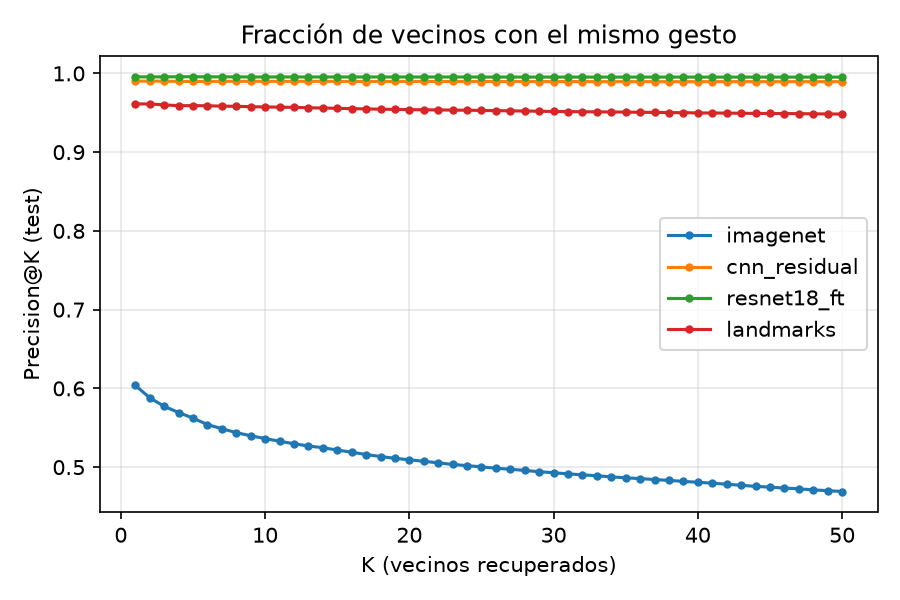
\includegraphics[width=0.6\textwidth]{precision_vs_k.png}
\caption{Precision@K en test para K de 1 a 50}
\fuente{Elaboración propia.}
\label{fig:pk}
\end{figure}

\textbf{El encoder del Hito 1 sirve para retrieval sin reentrenarlo.} Su mAP es 0.996, frente a
0.223 de la ResNet18 de ImageNet. Con ImageNet el vecino más parecido tiene el mismo gesto solo en
el 60\,\% de las consultas, y la precisión cae a medida que se recuperan más vecinos
(Figura~\ref{fig:pk}). Es lo mismo que mostró el linear probe del Hito 1, con 0.76 de macro F1: las
características de ImageNet no separan gestos que difieren en uno o dos dedos. La
Figura~\ref{fig:pca} lo muestra con PCA: con ImageNet los gestos forman una sola nube mezclada,
mientras que con el encoder ajustado cada gesto forma un grupo separado.

\begin{figure}[H]
\centering
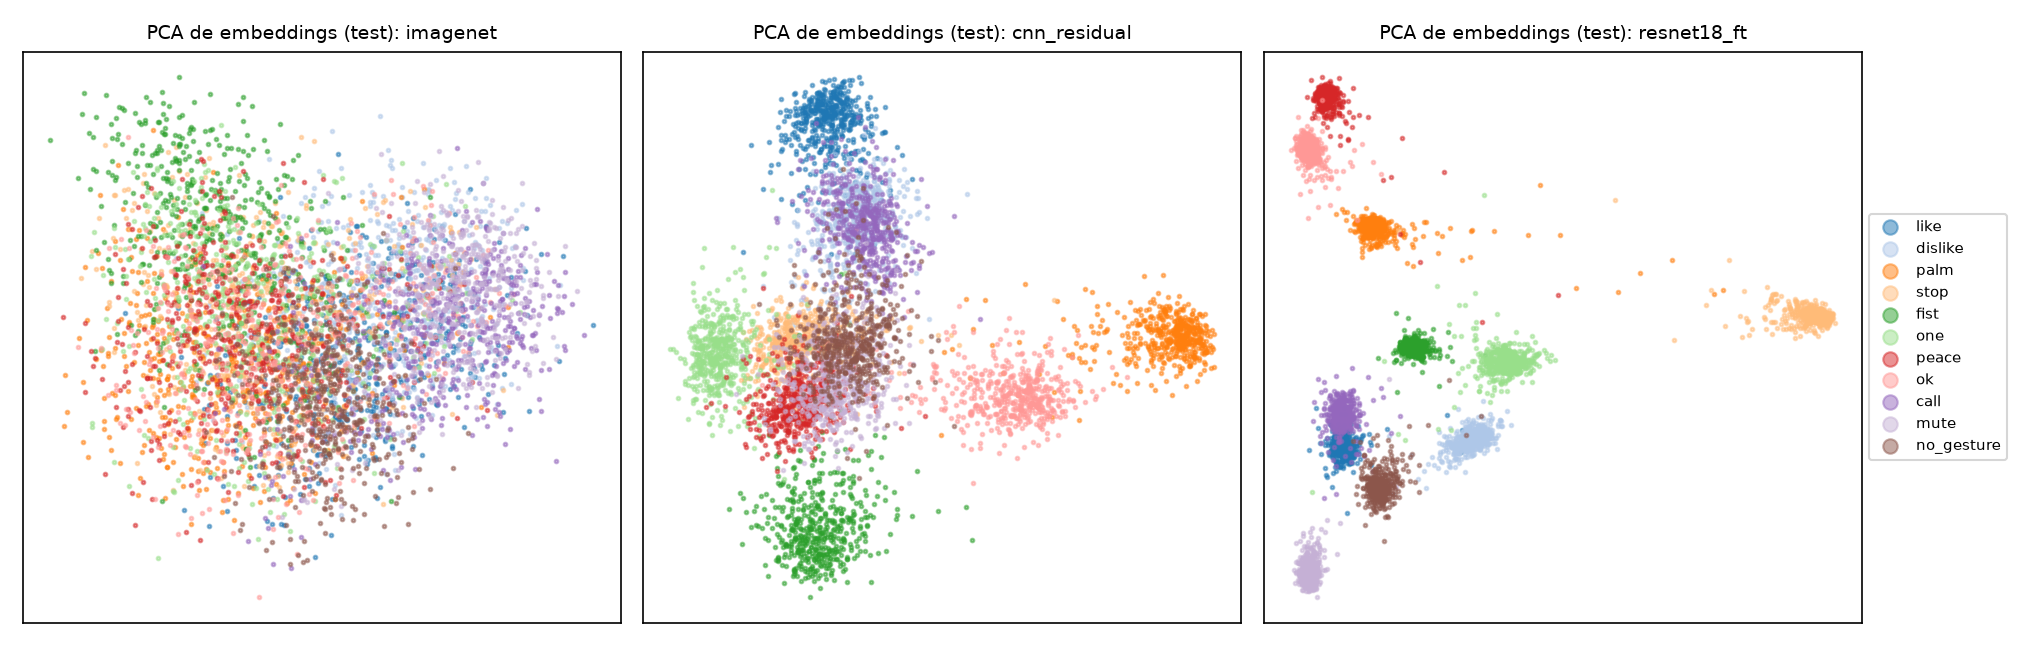
\includegraphics[width=\textwidth]{pca_embeddings.png}
\caption{Proyección PCA a dos dimensiones de los embeddings de test, coloreada por gesto}
\fuente{Elaboración propia.}
\label{fig:pca}
\end{figure}

\textbf{Buscar y votar es tan bueno como clasificar.} La votación de los 10 vecinos acierta el
99.5\,\% de los gestos, prácticamente igual que la cabeza de clasificación del Hito 1 (99.6\,\%), y
además entrega ejemplos parecidos que explican la decisión. La CNN propia queda muy cerca, con 0.986
de mAP y la mitad de dimensiones, lo que la hace una alternativa más barata de almacenar.

\textbf{Landmarks.} El vecino más parecido casi siempre acierta (R@1 de 0.961), pero el mAP es solo
0.519, es decir, muchas manos del mismo gesto quedan al final del ranking. Una explicación posible
es que la geometría centrada en la muñeca no es invariante a la rotación, por lo que un mismo gesto
forma varios grupos según la orientación de la mano. Esta hipótesis no se verificó.

\textbf{Errores.} La ResNet18 ajustada falla el vecino más parecido en 24 de 5\,500 consultas. Los
errores más frecuentes son \texttt{palm} recuperando \texttt{stop} (5), \texttt{call} recuperando
\texttt{no\_gesture}, \texttt{ok} recuperando \texttt{peace} y \texttt{peace} recuperando
\texttt{one} (3 cada uno), los mismos pares difíciles del Hito 1. Con ImageNet dominan
\texttt{peace} y \texttt{one} (249 casos entre ambas direcciones) y \texttt{ok} recuperando
\texttt{palm} (97). La Figura~\ref{fig:topk} muestra consultas acertadas y falladas.

\begin{figure}[H]
\centering
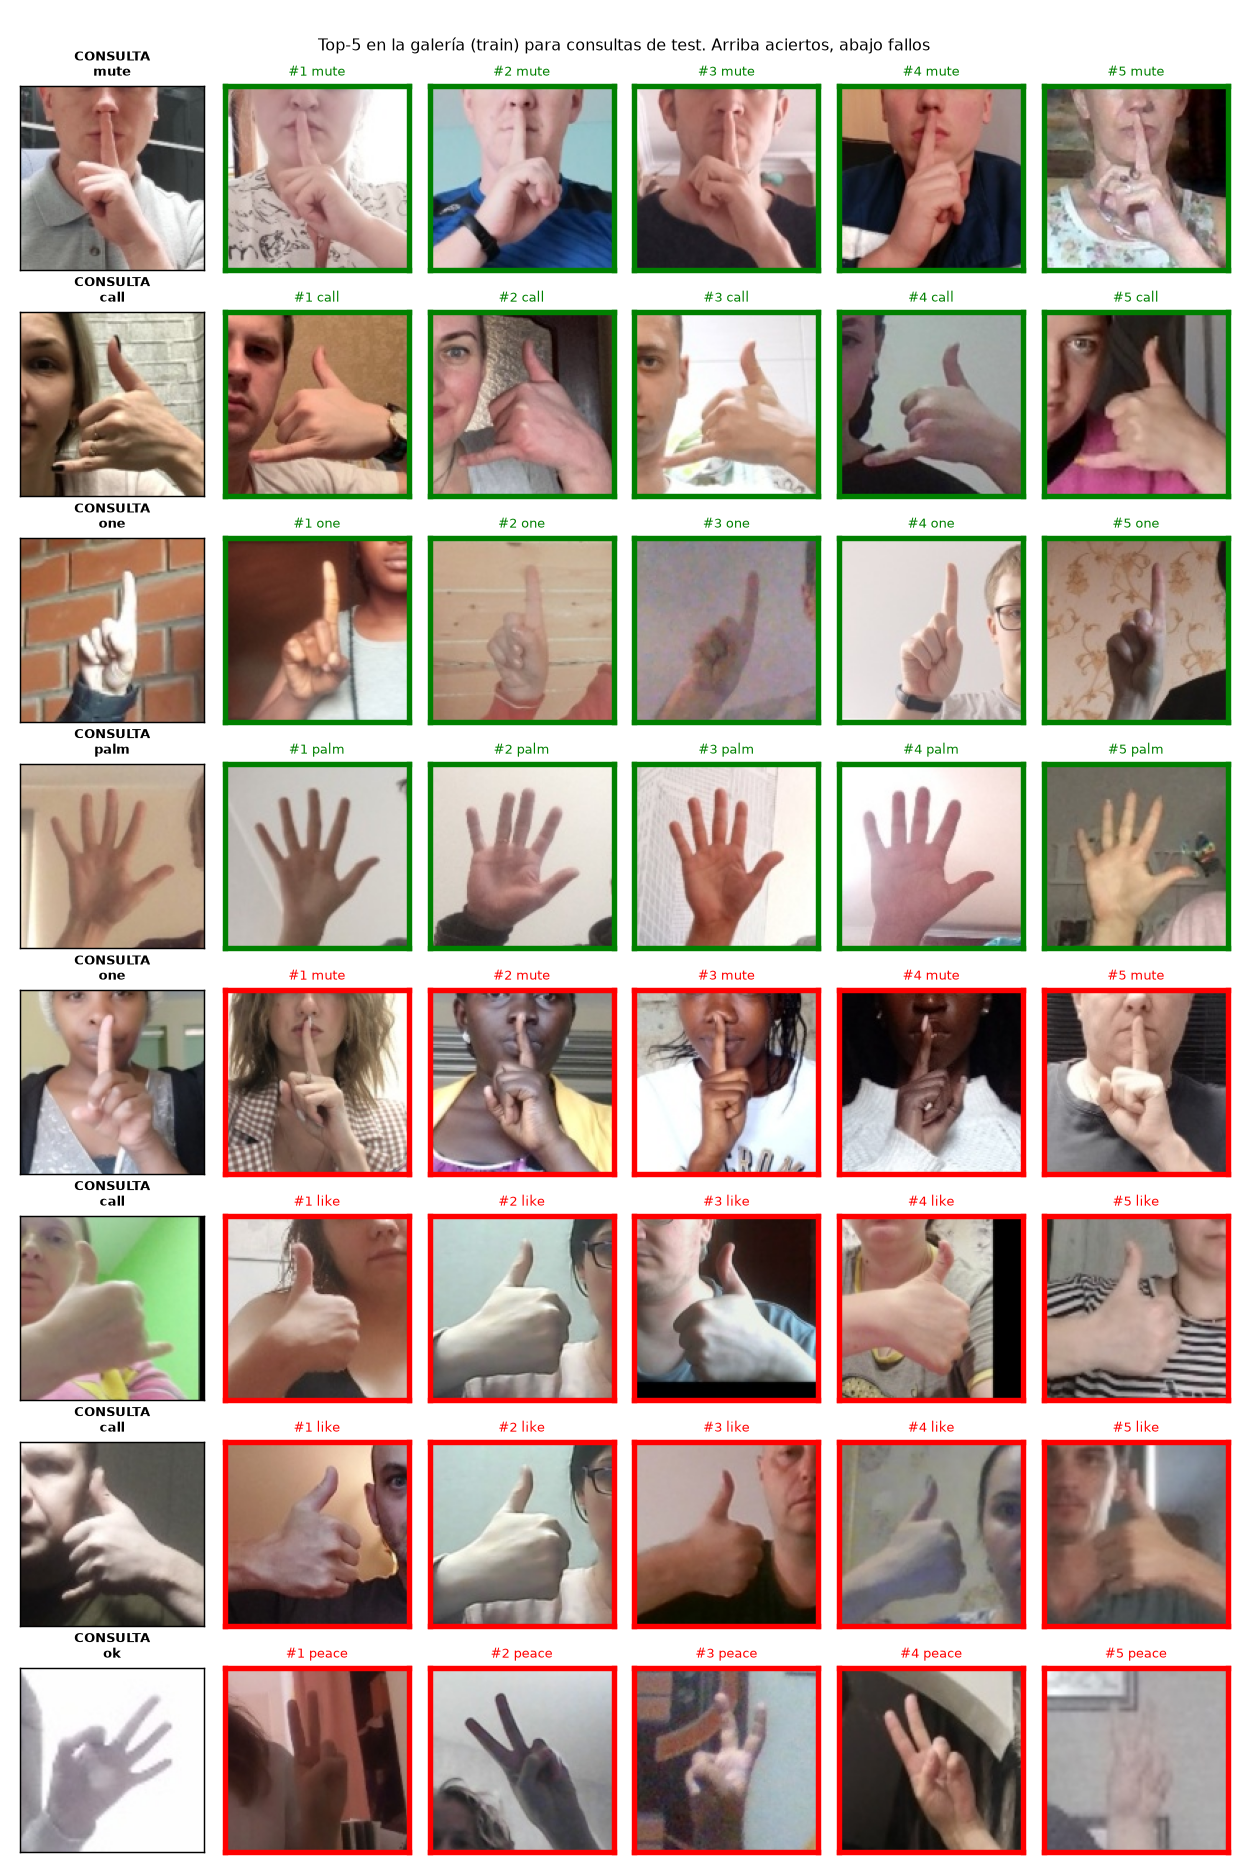
\includegraphics[height=0.66\textheight]{topk_resnet18_ft.png}
\caption{Consultas de test y sus 5 vecinos con el encoder elegido. Verde: mismo gesto; rojo: otro gesto}
\fuente{Elaboración propia a partir de imágenes de HaGRIDv2 \cite{hagridv2}.}
\label{fig:topk}
\end{figure}

\subsection{¿Gesto o identidad?}

El enunciado pide verificar que el embedding represente el gesto más que la identidad de la
persona. En la galería no se puede comprobar, porque ahí no hay nadie del test. Por eso el análisis
se hace dentro del test, donde cada persona aparece en varias fotos con gestos distintos. Para cada
mano se comparan las demás manos de test, excluyendo la otra mano de la misma foto, que tiene el
mismo fondo. Cada par cae en uno de cuatro grupos según si comparte gesto y si comparte persona
(Tabla~\ref{tab:identidad} y Figura~\ref{fig:identidad}). El grupo ``misma persona, mismo gesto'' son
casi siempre manos en reposo de otra foto de la misma persona.

\begin{table}[!htb]
\centering
\caption{Gesto frente a identidad en test}
\label{tab:identidad}
\begin{tabular}{lccc}
\toprule
 & ImageNet & CNN propia & ResNet18 ajustada \\
\midrule
Similitud media: mismo gesto, otra persona & 0.620 & 0.933 & \textbf{0.972} \\
Similitud media: misma persona, otro gesto & 0.616 & 0.566 & 0.560 \\
Similitud media: otra persona, otro gesto & 0.576 & 0.568 & 0.561 \\
\midrule
Top-10: misma persona con otro gesto (azar 0.0012) & \textbf{0.0295} & 0.0001 & 0.0000 \\
Consultas con la misma persona en su Top-10 & \textbf{22.3\,\%} & 0.11\,\% & 0.04\,\% \\
Percentil medio de la misma persona (50\,\% = azar) & \textbf{66\,\%} & 49.6\,\% & 49.4\,\% \\
\bottomrule
\end{tabular}
\fuente{Elaboración propia.}
\end{table}

\begin{figure}[H]
\centering
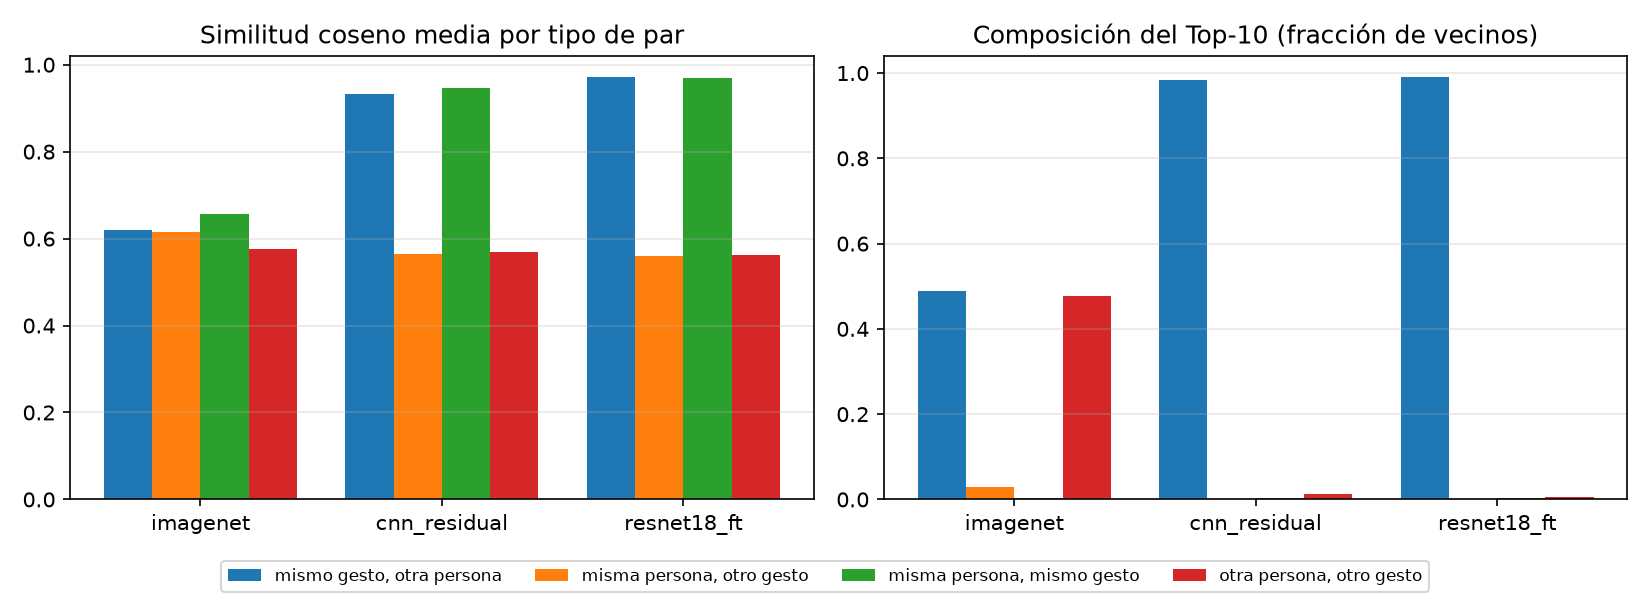
\includegraphics[width=\textwidth]{identidad_vs_gesto.png}
\caption{Similitud media por tipo de par y composición del Top-10 de cada consulta}
\fuente{Elaboración propia.}
\label{fig:identidad}
\end{figure}

\textbf{Con el encoder ajustado el embedding representa el gesto y no la persona.} La misma persona
haciendo otro gesto queda igual de lejos que un desconocido (similitud 0.560 frente a 0.561), y entre
las manos de otro gesto la mano de la misma persona queda en el percentil 49\,\%, lo mismo que al
azar. En cambio, con ImageNet sí se filtra identidad: la misma persona con otro gesto aparece en el
Top-10 25 veces más de lo que correspondería por azar, y en el 22\,\% de las consultas, porque la
foto comparte fondo, ropa y tono de piel (Figura~\ref{fig:identidad_ej}). El fine tuning del Hito 1
eliminó esa información porque no ayudaba a clasificar el gesto.

\begin{figure}[H]
\centering
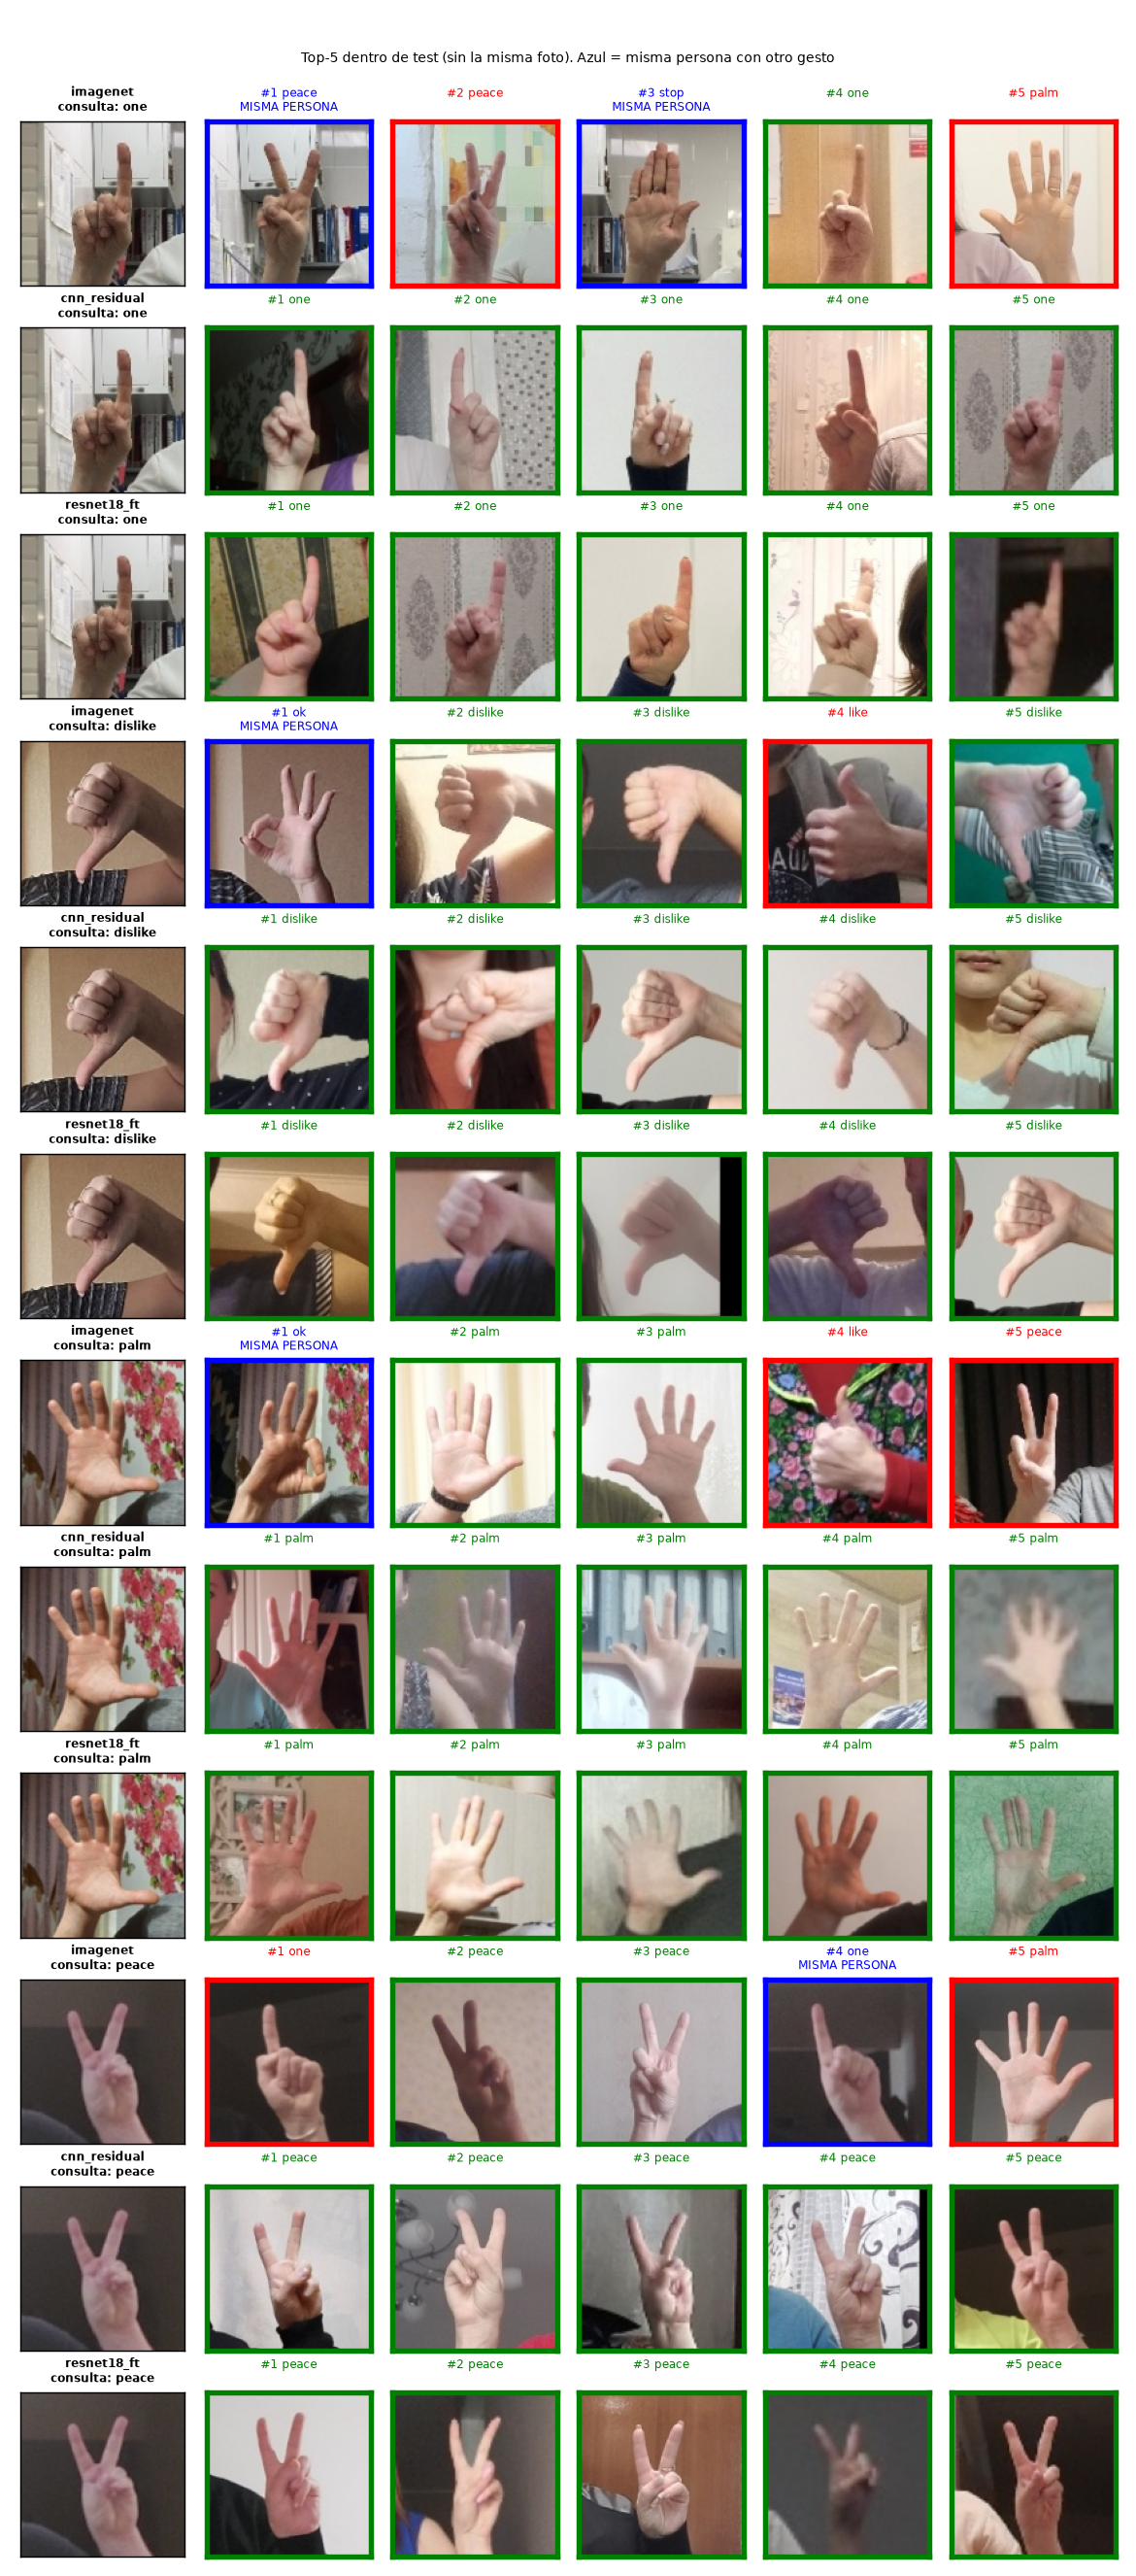
\includegraphics[height=0.7\textheight]{identidad_ejemplos.png}
\caption{Top-5 dentro de test, sin la misma foto. Borde azul: la misma persona con otro gesto}
\fuente{Elaboración propia a partir de imágenes de HaGRIDv2 \cite{hagridv2}.}
\label{fig:identidad_ej}
\end{figure}

\newpage
% =====================================================================================
\section{Sistema completo}

\subsection{Funcionamiento}

El sistema final une los tres hitos (Figura~\ref{fig:sistema}). El detector de manos del Hito 2
encuentra las manos con el umbral de confianza elegido en validación en ese hito (0.25). Cada mano se
recorta igual que en el Hito 1, como un cuadrado de 1.3 veces su lado mayor reducido a
$128 \times 128$ px, se calcula su embedding con el encoder elegido y se buscan sus 10 vecinos en la
galería. El gesto es el más votado entre ellos y de ahí sale el comando.

\begin{figure}[H]
\centering
\begin{tikzpicture}[node distance=0.35cm, every node/.style={font=\footnotesize, align=center},
    caja/.style={draw, rounded corners, minimum height=1cm, text width=1.7cm},
    flecha/.style={-{Stealth}, thick}]
\node[caja] (img) {Imagen};
\node[caja, right=of img, fill=orange!15] (det) {Detector de manos\\(Hito 2)};
\node[caja, right=of det] (crop) {Recorte\\$128\times128$};
\node[caja, right=of crop, fill=violet!15] (enc) {Encoder\\(Hito 1)};
\node[caja, right=of enc, fill=blue!10] (knn) {Top-10 en la galería};
\node[caja, right=of knn] (out) {Gesto por votación y comando};
\draw[flecha] (img) -- (det);
\draw[flecha] (det) -- (crop);
\draw[flecha] (crop) -- (enc);
\draw[flecha] (enc) -- (knn);
\draw[flecha] (knn) -- (out);
\end{tikzpicture}
\caption{Sistema final}
\fuente{Elaboración propia.}
\label{fig:sistema}
\end{figure}

Para saber el gesto real de cada caja detectada, se empareja con la mano real con la que más se
superpone, exigiendo un IoU de al menos 0.5. Las cajas sin pareja son falsos positivos y las manos
reales sin caja son manos perdidas, que cuentan como error en todas las métricas. Como referencia
se calcula el mismo retrieval con las cajas reales de las mismas 6\,049 manos, que es el techo del
sistema.

\subsection{Resultados}

\begin{table}[!htb]
\centering
\caption{Sistema completo en test frente al techo con cajas reales (6\,049 manos)}
\label{tab:sistema}
\begin{tabular}{lccccc}
\toprule
Sistema & mAP & R@1 & R@5 & P@10 & kNN10 acc. \\
\midrule
Techo: recorte con la caja real & 0.996 & 0.996 & 0.997 & 0.995 & 0.996 \\
\textbf{Detector + retrieval} & \textbf{0.955} & \textbf{0.954} & \textbf{0.956} & \textbf{0.954} & \textbf{0.954} \\
\bottomrule
\end{tabular}
\fuente{Elaboración propia.}
\end{table}

El sistema completo pierde 4.2 puntos de R@1 frente al techo (Tabla~\ref{tab:sistema}), y casi toda
la diferencia viene del detector. Se pierden 243 manos (4.0\,\%), y cuando la mano sí se detecta su
vecino más parecido tiene el gesto correcto en el 99.4\,\% de los casos, casi lo mismo que con la
caja real. Es decir, una vez encontrada la mano, el retrieval casi no se degrada.

\textbf{Distancia a la cámara.} Como en los hitos anteriores, el tamaño de la mano en píxeles se usó
como aproximación de la distancia (Tabla~\ref{tab:tamano}). Con las cajas reales el retrieval es
igual de bueno en los tres rangos, pero el sistema completo baja a 0.909 de R@1 en manos lejanas,
porque ahí ocurren 183 de las 243 manos perdidas.

\begin{table}[!htb]
\centering
\caption{R@1 en test por tamaño de la mano}
\label{tab:tamano}
\begin{tabular}{lcccc}
\toprule
Tamaño de la mano & Manos & Techo & Sistema & Manos perdidas \\
\midrule
Lejos, menor a 83 px & 2\,172 & 0.995 & 0.909 & 183 \\
Medio, 83 a 117 px & 1\,981 & 0.999 & 0.979 & 38 \\
Cerca, mayor a 117 px & 1\,896 & 0.994 & 0.981 & 22 \\
\bottomrule
\end{tabular}
\fuente{Elaboración propia.}
\end{table}

\textbf{Cajas mal centradas.} Entre las manos detectadas, el R@1 depende de qué tan bien la caja
calza con la mano (Tabla~\ref{tab:iou}). Con un IoU sobre 0.85 el sistema iguala al techo, pero
cuando el IoU está entre 0.5 y 0.7 baja a 0.971, frente a 0.992 con la caja real de esas mismas
manos. Un recorte desplazado puede cortar los dedos y cambiar el gesto que se ve, como el
\texttt{fist} que recupera manos \texttt{one} en la Figura~\ref{fig:casos}.

\begin{table}[!htb]
\centering
\caption{R@1 de las manos detectadas según el IoU de su caja}
\label{tab:iou}
\begin{tabular}{lccc}
\toprule
IoU de la caja detectada & Manos & Sistema & Techo con la caja real \\
\midrule
0.50 a 0.70 & 485 & 0.971 & 0.992 \\
0.70 a 0.85 & 2\,123 & 0.994 & 0.998 \\
0.85 a 1.00 & 3\,198 & 0.998 & 0.997 \\
\bottomrule
\end{tabular}
\fuente{Elaboración propia.}
\end{table}

\textbf{Falsos positivos.} El detector marca 344 cajas donde no hay una mano anotada. El 64\,\% de
ellas recupera manos \texttt{no\_gesture}, que no tienen comando asociado, por lo que no provocan
una acción. Además, su similitud con el vecino más parecido es menor que la de las manos reales,
0.937 frente a 0.990 en promedio, por lo que un umbral de similitud podría descartar parte de ellas.
Ese umbral no se fijó porque habría que elegirlo en validación.

\begin{figure}[H]
\centering
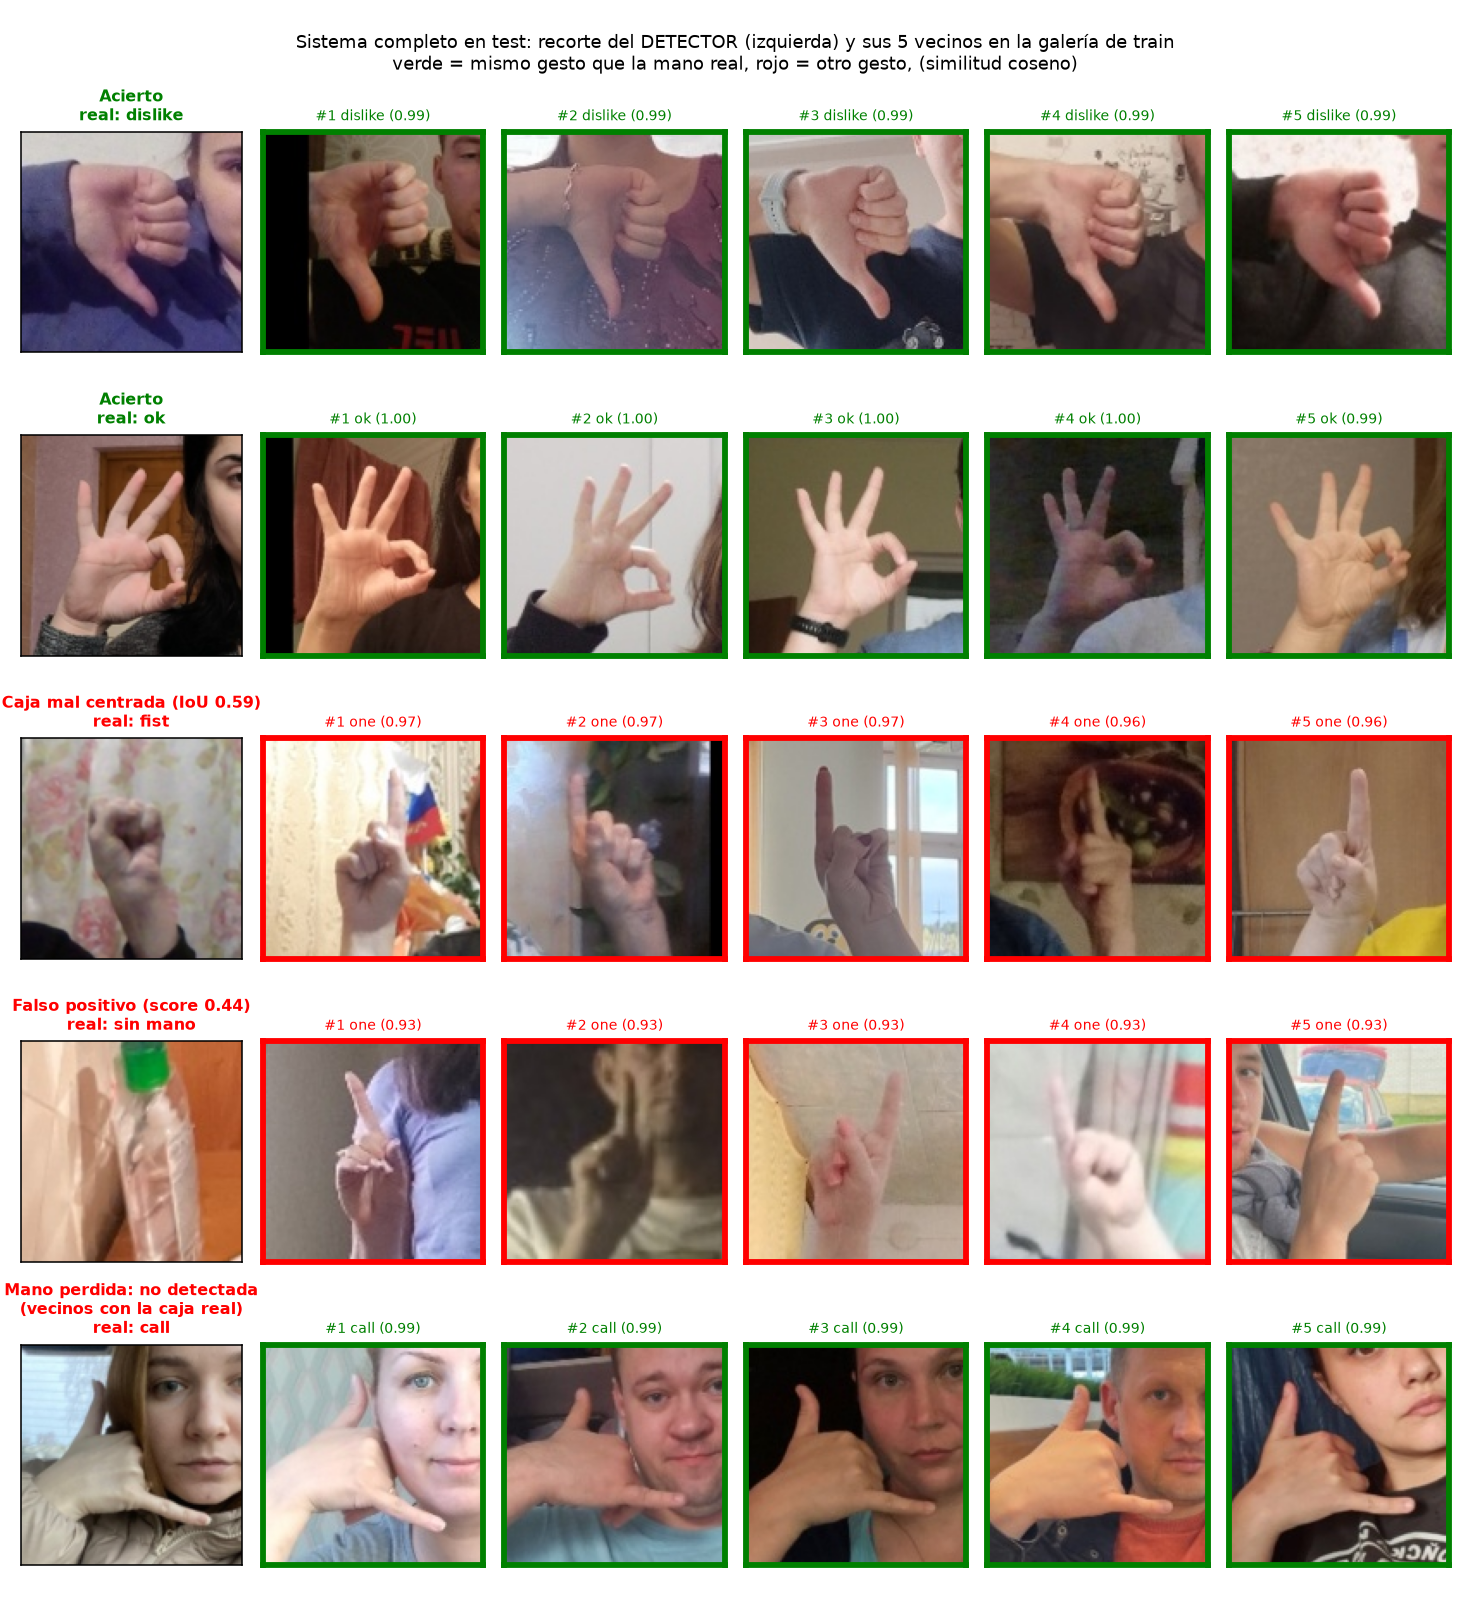
\includegraphics[width=0.85\textwidth]{casos_sistema.png}
\caption{Casos del sistema completo en test: aciertos, caja mal centrada, falso positivo y mano perdida}
\fuente{Elaboración propia a partir de imágenes de HaGRIDv2 \cite{hagridv2}.}
\label{fig:casos}
\end{figure}

\newpage
% =====================================================================================
\section{Demostración}

La demostración recibe una imagen y entrega, por cada mano, su caja, los 5 ejemplos más parecidos
de la galería, el gesto por votación y su comando. Los comandos son un ejemplo de control de un
dispositivo, como \texttt{like} para subir el volumen, \texttt{mute} para silenciar,
\texttt{peace} para cambiar al canal 2, \texttt{palm} para pausar o \texttt{ok} para confirmar. La
Figura~\ref{fig:demo} usa tres fotos externas al dataset tomadas por uno de los integrantes, en
formato horizontal y con un fondo distinto a los de HaGRIDv2. Los tres gestos se reconocen con los 10
votos y con vecinos de similitud entre 0.98 y 1.00. La Figura~\ref{fig:demo_test} muestra una imagen
de test con dos manos, donde la mano en reposo se reconoce como \texttt{no\_gesture} y no activa
ningún comando.

\begin{figure}[H]
\centering
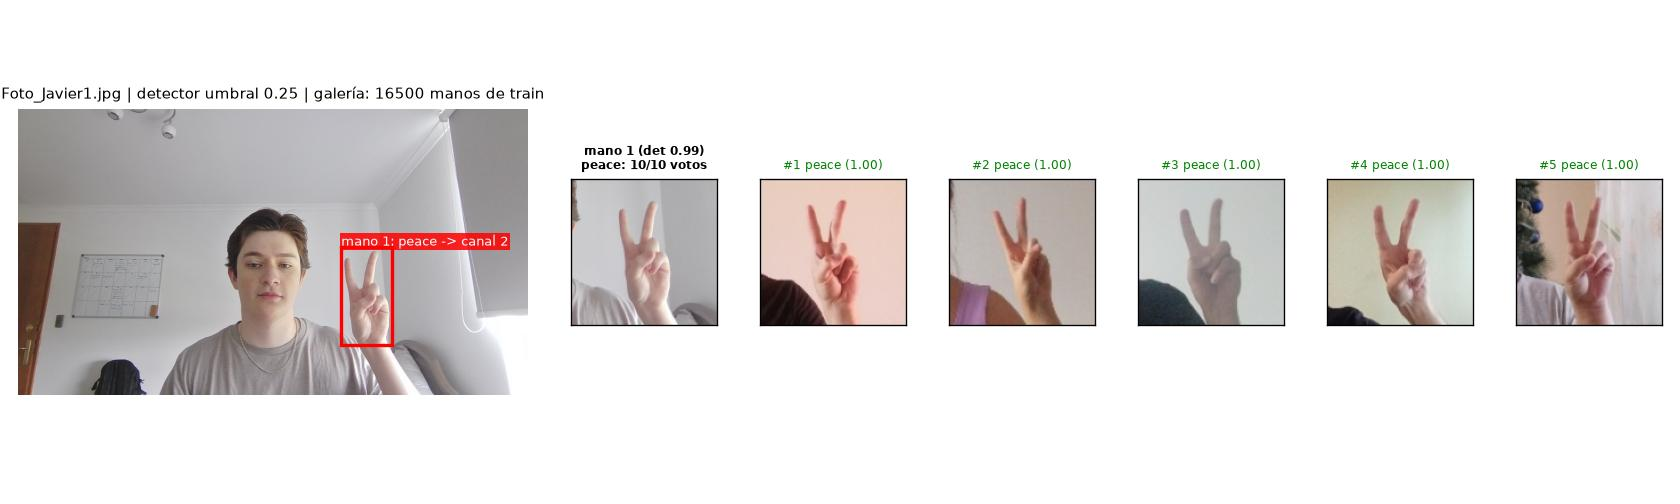
\includegraphics[width=0.86\textwidth,trim=0 45 0 0,clip]{Foto_Javier1_retrieval.jpg}\\
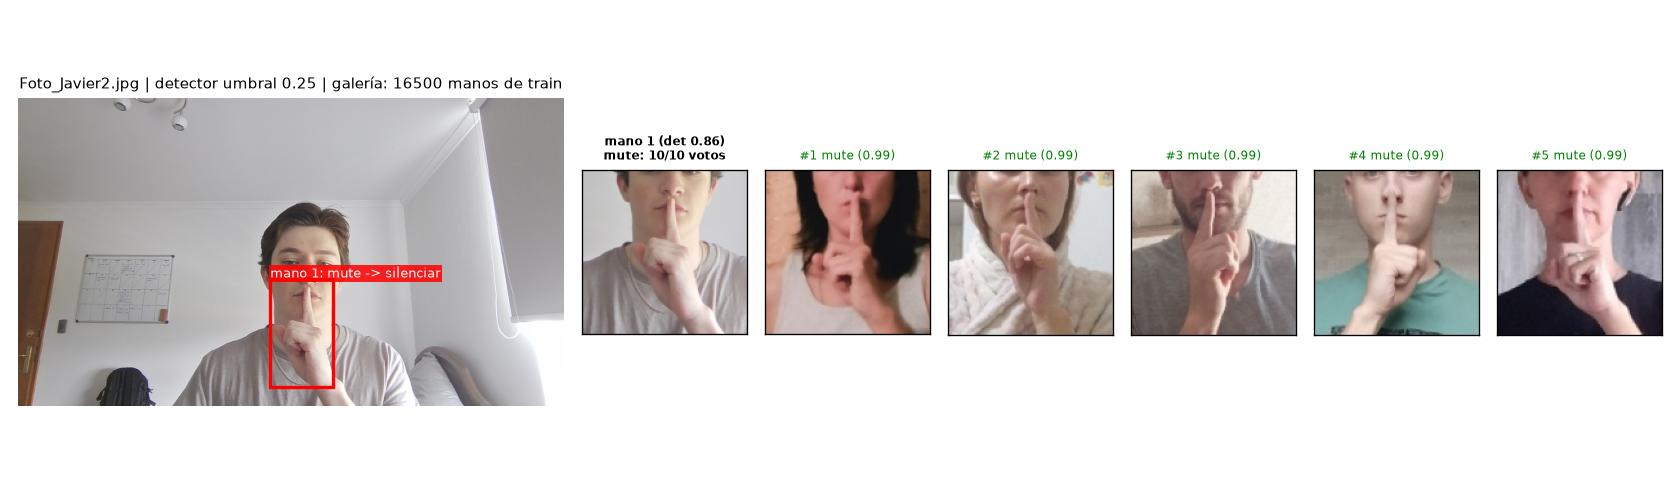
\includegraphics[width=0.86\textwidth,trim=0 45 0 0,clip]{Foto_Javier2_retrieval.jpg}\\
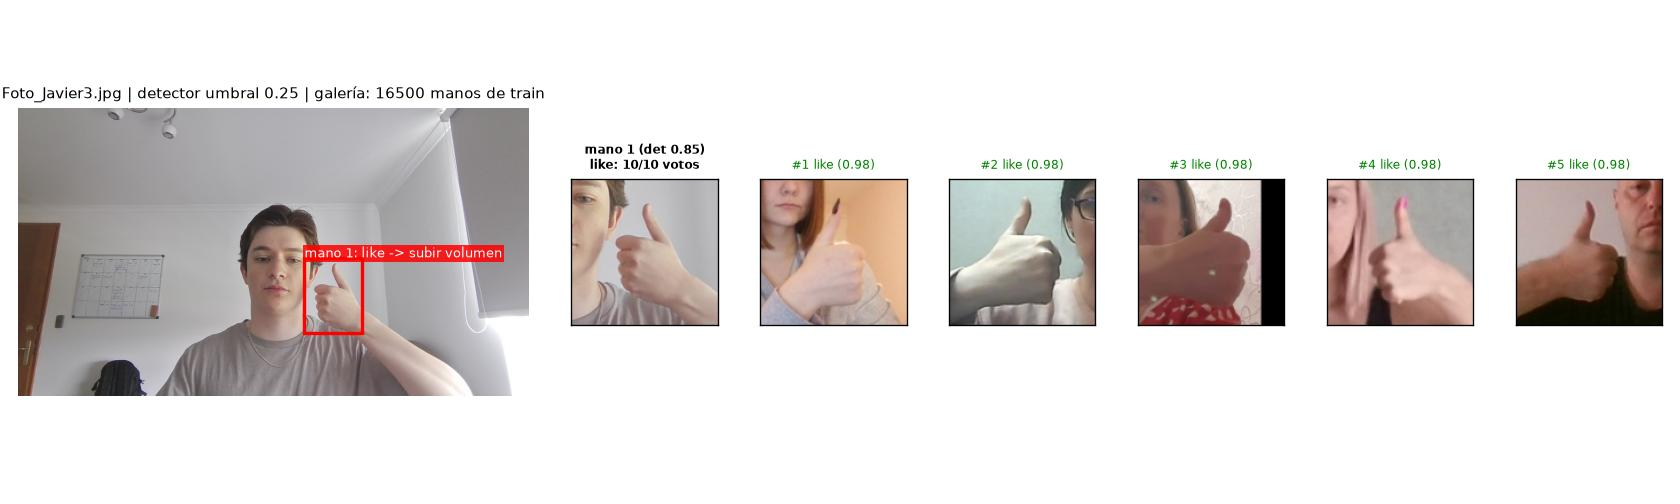
\includegraphics[width=0.86\textwidth,trim=0 45 0 0,clip]{Foto_Javier3_retrieval.jpg}
\caption{Demostración con fotos externas: mano detectada, gesto con sus votos, comando y 5 vecinos de la galería}
\fuente{Elaboración propia. Imágenes externas tomadas por los autores.}
\label{fig:demo}
\end{figure}

\begin{figure}[H]
\centering
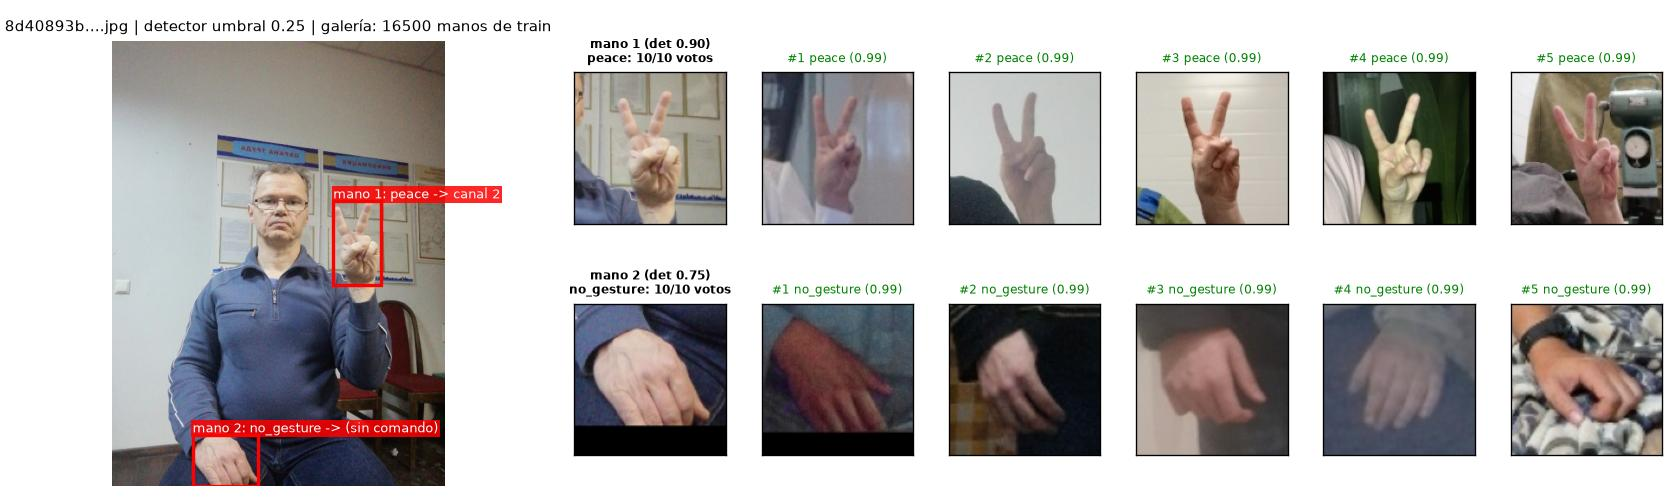
\includegraphics[width=\textwidth]{demo_test_dos_manos.jpg}
\caption{Demostración con una imagen de test con dos manos}
\fuente{Elaboración propia a partir de imágenes de HaGRIDv2 \cite{hagridv2}.}
\label{fig:demo_test}
\end{figure}

% =====================================================================================
\section{Conclusiones}

Se cumplió el objetivo del Hito 3. Se construyó el sistema completo imagen $\rightarrow$ detección
$\rightarrow$ recorte $\rightarrow$ embedding $\rightarrow$ Top-K, reutilizando sin reentrenar el
encoder del Hito 1 y el detector del Hito 2, con una galería y consultas de personas distintas.

El encoder del Hito 1 resultó una buena representación para buscar gestos, con 0.996 de mAP frente a
0.223 de una ResNet18 de ImageNet. Votar entre los vecinos es tan preciso como la cabeza de
clasificación del Hito 1 y además entrega ejemplos que explican la decisión.

El embedding representa el gesto y no la persona: con el encoder ajustado, la misma persona con otro
gesto queda tan lejos como un desconocido. Con ImageNet, en cambio, el 22\,\% de las consultas
recupera a la misma persona haciendo otro gesto.

Con las cajas del detector el sistema llega a 0.954 de R@1. La pérdida viene sobre todo de las manos
que el detector no encuentra, en su mayoría lejanas, y en menor medida de cajas mal centradas.
Una vez encontrada la mano, el retrieval casi no se degrada.

\textbf{Limitaciones.} La galería y las consultas provienen de HaGRIDv2, con una persona de frente en
interiores, y la demostración usa solo tres fotos externas de una misma persona. Las métricas del
sistema dependen del umbral del detector elegido en el Hito 2, y no se fijó un umbral de similitud
para descartar falsos positivos. Tampoco se midió el tiempo de ejecución ni se probó con video en
tiempo real.

\section*{Declaración de recursos externos}
\addcontentsline{toc}{section}{Declaración de recursos externos}

No se entrenaron modelos nuevos en este hito: se reutilizaron el encoder del Hito 1 y el detector de
manos del Hito 2. Para la comparación se usaron los pesos de ResNet18 preentrenada en ImageNet
incluidos en torchvision \cite{he2016}. La búsqueda por vecinos sigue la idea del clasificador KNN
visto en el curso. Las imágenes y anotaciones provienen de HaGRIDv2 \cite{hagridv2}, bajo licencia
CC BY SA 4.0, y las tres fotos de la demostración fueron tomadas por los autores. El código se
desarrolló con apoyo de un asistente de IA a partir del material del curso.

\begin{thebibliography}{9}
\addcontentsline{toc}{section}{Referencias}
\bibitem{hagridv2} A. Nuzhdin, A. Nagaev, A. Sautin, A. Kapitanov y K. Kvanchiani, ``HaGRIDv2: 1M Images for
Static and Dynamic Hand Gesture Recognition'', arXiv:2412.01508, 2024. Repositorio:
\url{https://github.com/hukenovs/hagrid}
\bibitem{he2016} K. He, X. Zhang, S. Ren y J. Sun, ``Deep Residual Learning for Image Recognition'',
\emph{IEEE Conference on Computer Vision and Pattern Recognition (CVPR)}, 2016.
\bibitem{repo} Repositorio del proyecto, \url{https://github.com/Melaooo/Proyecto-AI}
\end{thebibliography}

\newpage
\appendix
\section{Reproducibilidad}

El repositorio \cite{repo} incluye la partición congelada, los encoders del Hito 1 y el detector de
manos del Hito 2. Los embeddings de la galería se calculan la primera vez y se guardan en
\texttt{data/embeddings/}. Los resultados se reproducen con los siguientes comandos.

\begin{lstlisting}
python -m src.retrieval              # comparacion de encoders con cajas reales
python -m src.retrieval_identidad    # gesto frente a identidad
python -m src.retrieval_sistema      # sistema completo con el detector
python -m src.demo_retrieval --image demo/Foto_Javier1.jpg
python -m src.demo_retrieval --random 3
\end{lstlisting}

\end{document}
